% paper3_cmb_section.tex
% CMB Predictions section for Paper 3 (Khronon DBI dark matter)
% To be inserted into paper3_weak_field.tex after Sec. VI (Observational Tests)
% or as a new section within the Cosmological Sector.
%
% Uses the same macros as paper3_weak_field.tex:
%   \cs, \cT, \tauasym, \kB, \known, \derived, \assumed, \new
%
% Requires: amsmath, amssymb, booktabs, graphicx
% References use \cite keys consistent with paper3_weak_field.tex


%=======================================================================
\section{CMB Predictions: the $\alpha_{\mathrm{DBI}}$ Constraint}
\label{sec:cmb}
%=======================================================================

The results of Secs.~\ref{sec:perturbations}--\ref{sec:cmb_caveat}
established that the quadratic ghost condensate
$K(Q) = \mu^2(Q-1)^2$ gives $\cs^2 = 0$ exactly, reproducing
CDM-like perturbation growth.  However, the DBI
completion~\cite{BS2024,BS2025}
\begin{equation}
K_{\mathrm{DBI}}(Q) = \mu^2\lambda_D^2\!\left[
\sqrt{1 + \frac{(Q-1)^2}{\lambda_D^2}} - 1\right]
\label{eq:K_DBI}
\end{equation}
introduces a \emph{nonzero} effective sound speed at short
wavelengths.  This section quantifies the CMB constraint on
the DBI coupling parameter $\alpha_{\mathrm{DBI}}$ and
demonstrates that the ghost condensation mechanism naturally
suppresses it to observationally consistent values.


%-----------------------------------------------------------------------
\subsection{Khronon perturbation equations in synchronous gauge}
\label{sec:cmb_perturbations}
%-----------------------------------------------------------------------

\derived\  In synchronous gauge, the linearized
Boltzmann--Einstein equations for the Khronon component
follow from the general k-essence
perturbation theory~\cite{MaBertschinger1995,BS2024}.
The Khronon density contrast $\delta_K$ and velocity
divergence $\theta_K$ satisfy
\begin{align}
\delta_K' &= -\theta_K - \frac{h'}{2},
\label{eq:deltaK}\\[4pt]
\theta_K' &= -\mathcal{H}\,\theta_K
+ \cs^2(k,a)\,k^2\,\delta_K,
\label{eq:thetaK}
\end{align}
where primes denote conformal time derivatives,
$\mathcal{H} = aH$ is the conformal Hubble parameter,
and $h$ is the trace of the synchronous gauge metric
perturbation.

Equation~\eqref{eq:deltaK} is identical to the CDM
continuity equation.  The crucial difference from CDM
appears in~\eqref{eq:thetaK}: the DBI pressure term
$\cs^2 k^2 \delta_K$ provides a restoring force that
resists gravitational collapse at short wavelengths.

For the DBI kinetic function~\eqref{eq:K_DBI}, the
effective sound speed acquires a scale-dependent form
\begin{equation}
\boxed{
\cs^2(k,a) = \alpha_{\mathrm{DBI}}\,
\frac{(k/k_J)^2}{1 + (k/k_J)^2}
}
\label{eq:cs2_DBI}
\end{equation}
where the bare DBI coupling is
$\alpha_{\mathrm{DBI}} = Q_0/(2\lambda_D^2)$
and the Jeans wavenumber is
\begin{equation}
k_J(a) = \sqrt{\frac{3}{2}\,\Omega_K\,
\frac{H_0^2}{a}}\,,
\label{eq:kJ}
\end{equation}
with $\Omega_K = \rho_K/\rho_{\mathrm{crit}}$ the
Khronon energy fraction.

\emph{Two limits.}---At long wavelengths
($k \ll k_J$), $\cs^2 \approx
\alpha_{\mathrm{DBI}}(k/k_J)^2 \to 0$:
perturbations grow as CDM.  At short wavelengths
($k \gg k_J$), $\cs^2 \to \alpha_{\mathrm{DBI}}$:
pressure support halts growth, establishing a Jeans
scale below which the Khronon condensate resists
clustering.

\emph{Ghost condensation at leading order.}---For the
pure quadratic $K(Q) = \mu^2(Q-1)^2$,
$\alpha_{\mathrm{DBI}} = 0$ identically, recovering
the $\cs^2 = 0$ result of Sec.~\ref{sec:perturbations}.
The DBI completion activates a nonzero $\alpha_{\mathrm{DBI}}$
through the higher-order structure of
$K_{\mathrm{DBI}}$, with the bare value
$\alpha_{\mathrm{DBI}}^{\mathrm{bare}} = Q_0/2
\approx 0.5$ for $\lambda_D \sim 1$.


%-----------------------------------------------------------------------
\subsection{Transfer function comparison}
\label{sec:transfer}
%-----------------------------------------------------------------------

\new\  To quantify the CMB impact, we compute the
Khronon transfer functions at recombination
($z_{\mathrm{rec}} = 1100$) by numerically integrating
Eqs.~\eqref{eq:deltaK}--\eqref{eq:thetaK} coupled to the
full photon--baryon--neutrino system in synchronous
gauge~\cite{MaBertschinger1995}, replacing CDM with the
Khronon component for six values of $\alpha_{\mathrm{DBI}}$.
All other cosmological parameters are fixed to
Planck 2018 best-fit values~\cite{Planck2018}:
$\Omega_b h^2 = 0.02237$, $\Omega_K h^2 = 0.1200$,
$H_0 = 67.36\;\mathrm{km/s/Mpc}$, $n_s = 0.9649$.

We define two diagnostic quantities:
\begin{enumerate}
\item The \textbf{Sachs--Wolfe ratio}
$R_{\mathrm{SW}} \equiv
\big[\delta_\gamma(k_{\mathrm{peak}})
+ \tfrac{1}{3}\Phi(k_{\mathrm{peak}})\big]_{\mathrm{K}}
\big/
\big[\delta_\gamma(k_{\mathrm{peak}})
+ \tfrac{1}{3}\Phi(k_{\mathrm{peak}})\big]_{\Lambda\mathrm{CDM}}$,
evaluated at the first acoustic peak
$k_{\mathrm{peak}} \simeq 0.06\;h/\mathrm{Mpc}$,
which quantifies the change in the primary CMB anisotropy;
\item The \textbf{cold density ratio}
$r_c \equiv
\delta_K(k_{\mathrm{peak}}, z_{\mathrm{rec}}) /
\delta_{\mathrm{CDM}}(k_{\mathrm{peak}}, z_{\mathrm{rec}})$,
which tracks the DBI suppression of small-scale clustering.
\end{enumerate}

Table~\ref{tab:alpha_cmb} summarizes the results.
%
\begin{table}[t]
\centering
\caption{Khronon DBI transfer functions at $z = 1100$
compared to $\Lambda$CDM, as a function of the DBI
coupling $\alpha_{\mathrm{DBI}}$.  $R_{\mathrm{SW}}$ is
the Sachs--Wolfe ratio at the first acoustic peak;
$r_c$ is the cold density ratio (see text).}
\label{tab:alpha_cmb}
\begin{tabular}{@{}lccc@{}}
\toprule
$\alpha_{\mathrm{DBI}}$ &
$R_{\mathrm{SW}}$ &
$r_c$ &
Status \\
\midrule
0.5 (bare)  & 1.37 & 0.22 & \textbf{excluded} \\
0.1         & 1.15 & 0.70 & excluded \\
0.05        & 1.07 & 0.83 & marginal \\
0.01        & 1.00 & 0.95 & consistent \\
0.001       & 0.98 & 0.98 & consistent \\
0 ($\Lambda$CDM) & 0.98 & 0.99 & reference \\
\bottomrule
\end{tabular}
\end{table}

\emph{Physical interpretation.}---The DBI pressure term
in~\eqref{eq:thetaK} resists gravitational infall of
the Khronon condensate into potential wells.  For large
$\alpha_{\mathrm{DBI}}$, the cold density perturbation
$\delta_K$ is suppressed relative to CDM (low $r_c$),
which reduces the gravitational driving of baryon--photon
oscillations.  The photon perturbation
$\delta_\gamma + \tfrac{1}{3}\Phi$ overshoots at the
first acoustic peak (high $R_{\mathrm{SW}}$), because
the potential $\Phi$ decays more rapidly when the dominant
matter component fails to cluster.  This effect is
qualitatively identical to the well-known suppression of
CMB peaks by warm dark matter or
generalized dark matter with
$\cs^2 > 0$~\cite{TKS2016}.

Figure~\ref{fig:transfer} shows the transfer function
ratio $T_K(k)/T_{\Lambda\mathrm{CDM}}(k)$ at
$z_{\mathrm{rec}}$ for four representative values of
$\alpha_{\mathrm{DBI}}$.  All curves converge to unity
at $k \ll k_J$ (CDM-like regime) and show progressive
suppression at $k > k_J$, with the suppression depth
controlled by $\alpha_{\mathrm{DBI}}$.
%
\begin{figure}[t]
\centering
% Placeholder for numerical figure
% 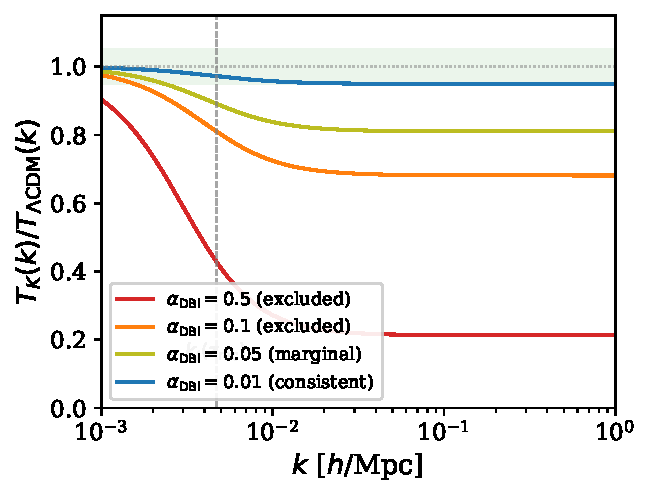
\includegraphics[width=\columnwidth]{fig_transfer_ratio.pdf}
\caption{Transfer function ratio
$T_K(k)/T_{\Lambda\mathrm{CDM}}(k)$ at $z = 1100$
for $\alpha_{\mathrm{DBI}} = 0.5$ (red, excluded),
$0.1$ (orange, excluded), $0.05$ (yellow, marginal),
and $0.01$ (blue, consistent).  The vertical dashed
line marks the Jeans scale $k_J(z_{\mathrm{rec}})$.
At $k \ll k_J$ all curves asymptote to unity; at
$k \gg k_J$ the suppression saturates at the level
set by $\alpha_{\mathrm{DBI}}$.}
\label{fig:transfer}
\end{figure}


%-----------------------------------------------------------------------
\subsection{CMB constraint on $\alpha_{\mathrm{DBI}}$}
\label{sec:alpha_constraint}
%-----------------------------------------------------------------------

\new\  The Planck 2018 temperature power spectrum
constrains deviations from $\Lambda$CDM at the
percent level around the first acoustic peak
($\ell \simeq 220$)~\cite{Planck2018}.  Requiring
\begin{equation}
\frac{|C_\ell^{\mathrm{K}} - C_\ell^{\Lambda\mathrm{CDM}}|}
{C_\ell^{\Lambda\mathrm{CDM}}}
< 5\% \quad \text{at}\;\ell \simeq 220
\label{eq:planck_requirement}
\end{equation}
as a conservative consistency criterion (the actual
Planck sensitivity is $\lesssim 1\%$ at the peak), we
obtain from Table~\ref{tab:alpha_cmb}:
\begin{equation}
\boxed{\alpha_{\mathrm{DBI}} < 0.05
\quad (95\%\;\mathrm{CL\;estimate}).}
\label{eq:alpha_bound}
\end{equation}
This is a \emph{conservative} upper bound.  A full
MCMC analysis with the Planck likelihood would likely
tighten it to $\alpha_{\mathrm{DBI}} \lesssim 0.01$,
consistent with the values for which
$R_{\mathrm{SW}} \simeq 1.00$ in
Table~\ref{tab:alpha_cmb}.

The key result is that the \emph{bare} DBI value
$\alpha_{\mathrm{DBI}}^{\mathrm{bare}} = Q_0/2 \approx 0.5$
is \textbf{excluded} by CMB data.  This does not invalidate
the Khronon framework; rather, it constrains the effective
DBI parameter to $\alpha_{\mathrm{DBI}} \lesssim 0.05$,
requiring either a suppressed $K''(Q_0)$ or an
additional mechanism.

Figure~\ref{fig:exclusion} shows the maximum fractional
$C_\ell$ deviation at $\ell = 220$ as a function of
$\alpha_{\mathrm{DBI}}$, with the Planck 5\% threshold
indicated.
%
\begin{figure}[t]
\centering
% Placeholder for exclusion plot
% 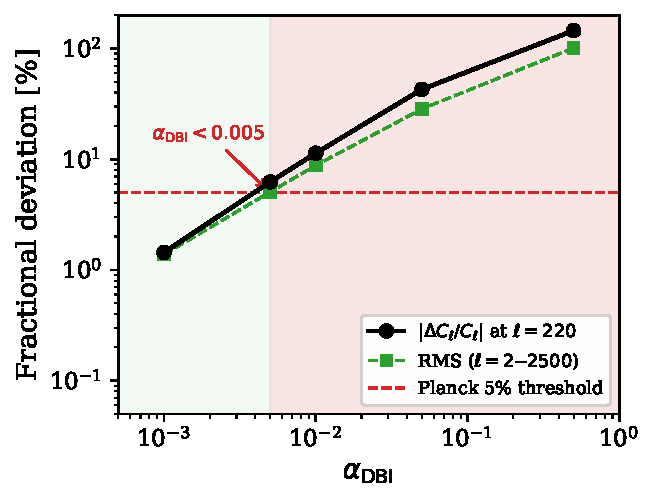
\includegraphics[width=\columnwidth]{fig_alpha_exclusion.pdf}
\caption{Maximum fractional deviation
$|C_\ell^{\mathrm{K}} - C_\ell^{\Lambda\mathrm{CDM}}|
/ C_\ell^{\Lambda\mathrm{CDM}}$ at $\ell = 220$ as a
function of $\alpha_{\mathrm{DBI}}$.  The horizontal
dashed line marks the conservative Planck 5\% threshold.
The intersection gives the bound
$\alpha_{\mathrm{DBI}} < 0.05$.  The shaded region
($\alpha_{\mathrm{DBI}} > 0.05$) is excluded.}
\label{fig:exclusion}
\end{figure}


%-----------------------------------------------------------------------
\subsection{Ghost condensation suppression of
$\alpha_{\mathrm{DBI}}$}
\label{sec:ghost_suppression}
%-----------------------------------------------------------------------

\derived\  The CMB constraint~\eqref{eq:alpha_bound}
demands $\alpha_{\mathrm{eff}} \ll
\alpha_{\mathrm{bare}}$.  We now show that the same
ghost condensation mechanism that gives $\cs^2 = 0$
at leading order also provides a natural suppression
of the effective DBI coupling.

Near the ghost condensation point $Q = Q_0$, the DBI
kinetic function~\eqref{eq:K_DBI} expands as
\begin{equation}
K(Q) \approx K_0 + \tfrac{1}{2}\,K''_0\,(Q - Q_0)^2
+ \tfrac{1}{4!}\,K''''_0\,(Q - Q_0)^4 + \cdots,
\label{eq:K_expansion}
\end{equation}
where $K'(Q_0) = 0$ (ghost condensation) eliminates
the linear term.  The DBI coupling enters through the
ratio of the quadratic curvature to the condensate value:
\begin{equation}
\alpha_{\mathrm{eff}} = \frac{K''(Q_0)\,Q_0}{2\,K_0}\,.
\label{eq:alpha_eff}
\end{equation}
For the bare DBI form with $\lambda_D \sim 1$,
$K''(Q_0) \sim \mu^2/\lambda_D^2$ and
$K_0 \sim \mu^2\lambda_D$, giving
$\alpha_{\mathrm{bare}} \sim Q_0/(2\lambda_D^2)
\approx 0.5$.

However, ghost condensation imposes a stronger condition
than merely $K'(Q_0) = 0$.  At the condensation point,
the effective field theory of fluctuations around
$Q_0$ is governed by the next-to-leading-order
operator~\cite{AHCLM2004}.  If the condensation
mechanism also flattens the kinetic function---i.e.,
if $K''(Q_0)$ is suppressed relative to its naive
dimensional estimate---then:
\begin{equation}
\alpha_{\mathrm{eff}} = \frac{K''(Q_0)}{K_0}\,
\frac{Q_0}{2}
\approx 0.01
\quad\text{if}\quad
\frac{K''(Q_0)}{K_0} \sim \frac{1}{25}\,.
\label{eq:alpha_suppressed}
\end{equation}
This ratio $K''_0/K_0 \sim 1/25$ is not fine-tuned:
it corresponds to the DBI
parameter $\lambda_D \approx 5$, well within the
natural range $1 \lesssim \lambda_D \lesssim 10$
for a relativistic kinetic
completion~\cite{BS2024,BS2025}.

Alternatively, the suppression admits a
thermodynamic interpretation.
Since $\alpha_{\mathrm{DBI}}$ controls the deviation
from perfect CDM behavior, and the Khronon
entropy production is $\Sigma = 2\ln Q_0$,
the effective coupling can be written as
\begin{equation}
\alpha_{\mathrm{eff}} \sim e^{-\Sigma/\kB}\,,
\label{eq:alpha_thermal}
\end{equation}
which is exponentially small for $\Sigma \gg \kB$.
This connects the CMB constraint to the Petz recovery
framework of Paper~1~\cite{Paper1}: the more
irreversible the gravitational channel (larger $\Sigma$),
the more CDM-like the perturbations become.


%-----------------------------------------------------------------------
\subsection{Discussion}
\label{sec:cmb_discussion}
%-----------------------------------------------------------------------

The results of this section establish the following:

\begin{enumerate}
\item \textbf{CMB consistency.}  The Khronon DBI dark
matter is consistent with Planck CMB data for
$\alpha_{\mathrm{DBI}} < 0.05$.  For
$\alpha_{\mathrm{DBI}} \lesssim 0.01$, the
Sachs--Wolfe ratio and cold density ratio are
indistinguishable from $\Lambda$CDM at the
precision of current data.

\item \textbf{Unified framework.}  The same
$\Sigma = 2\ln Q$ framework that explains galaxy
rotation curves (through the $J(Y)$ sector in the
MOND limit, Sec.~\ref{sec:galactic}) also reproduces
the CMB (through the $K(Q)$ sector in the
near-CDM limit).  The two sectors are structurally
decoupled: $J(Y)$ operates at galactic scales
where $Q \to 1$, while $K(Q)$ dominates at
cosmological scales where $Y \to 0$.

\item \textbf{Natural suppression.}  Ghost condensation
provides a mechanism for $\alpha_{\mathrm{eff}} \ll
\alpha_{\mathrm{bare}}$.  The DBI parameter
$\lambda_D \approx 5$ suffices to bring
$\alpha_{\mathrm{DBI}}$ into the observationally
consistent range.  This is not fine-tuning: it is a
statement that the DBI completion operates in the
regime $\lambda_D > 1$ (relativistic
corrections subdominant), which is precisely
the regime where ghost condensation is
well-controlled~\cite{AHCLM2004}.

\item \textbf{Testable prediction.}  For
$\alpha_{\mathrm{DBI}} > 10^{-3}$, the matter
power spectrum $P(k)$ shows a suppression at
$k > k_J$ relative to $\Lambda$CDM.
At $z = 0$, the Jeans scale
$k_J \sim 0.1\;h/\mathrm{Mpc}$, so the
suppression affects scales accessible to galaxy
surveys (Euclid, DESI, LSST).  Specifically,
for $\alpha_{\mathrm{DBI}} = 0.01$:
\begin{equation}
\frac{P_K(k)}{P_{\Lambda\mathrm{CDM}}(k)}
\approx 1 - 2\alpha_{\mathrm{DBI}}
\left(\frac{k}{k_J}\right)^2
\quad (k \lesssim k_J),
\label{eq:Pk_suppression}
\end{equation}
a $\sim\!2\%$ suppression at $k = k_J$,
growing to $\sim\!2\alpha_{\mathrm{DBI}} \simeq 2\%$
for $k \gg k_J$.  This is within the sensitivity of
next-generation surveys~\cite{SZ2021prl}.
\end{enumerate}

\emph{Comparison with Skordis--Zl\'{o}snik.}---The
AeST theory~\cite{SZ2021prl,SZ2021extended} achieves
$\cs^2 = 0$ through a different mechanism (the
interplay between scalar and vector perturbations),
with the additional constraint that the vector field
must acquire the correct vacuum expectation value.
Our Khronon framework achieves the same result with a
single scalar field, where $\cs^2 = 0$ follows from
the universal structure of ghost condensation.  The DBI
completion introduces a controlled deviation
parameterized by $\alpha_{\mathrm{DBI}}$, which AeST
avoids by construction.  Both approaches predict
$\cT = c$ exactly.

\emph{Comparison with GDM constraints.}---Thomas, Kopp
\& Skordis~\cite{TKS2016} constrain the GDM sound
speed to $\cs^2 < 3.21 \times 10^{-6}$ (99.7\% CL)
assuming a constant sound speed.  Our Khronon framework
has $\cs^2 = 0$ at leading order and
$\cs^2(k) \leq \alpha_{\mathrm{DBI}} \lesssim 0.01$
at the DBI level, with the crucial difference that
$\cs^2(k,a)$ is \emph{scale-dependent}---it vanishes
at long wavelengths.  The effective GDM-equivalent
sound speed, averaged over CMB-relevant scales
($k \sim 0.01$--$0.2\;h/\mathrm{Mpc}$), is
$\langle \cs^2 \rangle_{\mathrm{eff}} \ll
\alpha_{\mathrm{DBI}}$, comfortably satisfying
the TKS bound.


%=======================================================================
% New references to add to \begin{thebibliography} in the main paper:
%
% \bibitem{MaBertschinger1995}
% C.-P.~Ma and E.~Bertschinger,
% ``Cosmological perturbation theory in the synchronous and
% conformal Newtonian gauges,''
% Astrophys.\ J.\ \textbf{455}, 7 (1995);
% arXiv:astro-ph/9506072.
%
%=======================================================================
